\chapter{\textbf{System Methodology}}
A system development methodology refers to the framework that is used to structure, plan, and control the process of developing an information system. Each of the available methodologies is best suited to specific kinds of projects, based on various technical, organizational, project and team considerations.
\section{System Overview}
In this thesis, environment monitoring systems is implemented by using sensors and then send the sensors data are sent to a local internet protocol (IP) using Wi-Fi. For enchanting data, DHT-11 (Temperature and Humidity sensor) and MQ-6 (LPG gas sensor) are being used. The basic objective of this work is to monitor and to develop a real-time monitoring of humidity and temperature, as well as the availability of gas using the very available DHT-11 sensor, MQ-6 sensor, and ESP-8266 NodeMCU module and then observe the data from a local IP based webpage. In this, a system has been developed to monitor the real-time condition (Humidity and Temperature to be more precise) through a local IP without the access of internet, because of security reason and so on; in which physical presence is not needed.
\begin{figure}[h]
\vspace{.5in}
  \centering
  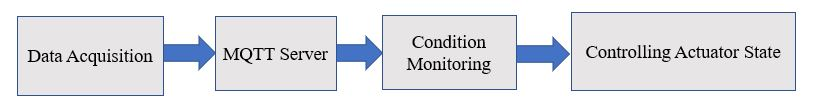
\includegraphics[width=6in]{12}
  \caption{ System Block Diagram}\label{fig12}
  \vspace{.5in}
\end{figure}
Node MCU is a kind of component that consists of an ESP8266 Wi-Fi along with a microcontroller with 1 analog and 12 digital pins, for which it is more efficient than an Arduino board and the data rate is also effective for this module. Combining the results with MATLAB environment, the upcoming data can also be forecasted through the basic knowledge of MATLAB or other engineering and scientific software. However, using an Arduino board is not necessary for just monitoring services, because of cost management and time consumption. This work has been directed using very modest methodology and appliances which are available and require minimal technical knowledge to operate. It discusses one of the implementations of a system using Wireless Sensor Networking (WSN). MQ-2 gas sensor and IR photodiode are used to determine smoke/gas concentration and fire presence respectively. As the gas sensor works fine within temperature ranging 2535 0C \& RH ranging 55-70\%, so DHT-11 sensor is used to check the temperature and relative humidity level of the experimental plant. Further mathematical modeling and analysis are done for the steady-state design of the experimental system. After that acquisition of those factors which combines a threshold, value has to be set for controlling the total system modeling. From the datasheet of DHT-11, MQ-2 and IR photodiode, parameters and the operations are obtained. The DHT-11 sensor is a digital sensor with digital output data, which combines Integrated Circuits, is the reason behind the direct values of relative humidity and temperature can be obtained.

\section{Why ESP8266 is Used}
In this project work we have used ESP8266 as MCU because of the following reasons:\\\\
\textbf{(i)Ideal Stuff for IoT and WSN:} ESP8266 is ideal for Internet of Things (IoT) My current project involves home automation and IoT stuff. It would send the status of a PIR Sensor over WIFI to an MQTT broker every 2.5 seconds. With built-in WIFI, these boards are ideal for Internet activities.\\\\
\textbf{(ii)Programmable PWM Frequency:} The ESP8266 core of the Arduino library, however, has a built-in PWM frequency call. The ESP8266 core has 1024 (0-1023) levels of pulse-width instead of Arduino’s 256 (0-255). One option is to change the PWM frequency, but that would mean digging in the Arduino libraries.\\\\
\textbf{(iii)Any pins can be selected for I2C:} A simple call before initializing the wire library allows for I2C communication on any of the module’s pins.\\\\
\textbf{(iv)Works with Arduino IDE:} The reason for choosing this is that the ESP8266 works well with the Arduino IDE.\\\\
\textbf{(v)Inexpensive:} The Adafruit ESP8266 boards have incredible build quality, nice features (like all the necessary pull-ups), and support a company that supports the maker community in countless ways. Moreover, it is cheap in price.

\section{System Flowchart}
Firstly, when the Node MCU is turned, it first runs the program compiled in it and starts calibrating the sensors. On concluding calibration, it first goes to connect the local server via triggering its Tx and Rx. Now, two types of conditions are relevant; at calibration, the controller detects any problem in sensor value then it sends a signal to the control unit and commands it to make an action. Next, it starts recalibration and if no defect is found then it tries to connect the hotspot which is specified in the program and it checks for the preprogrammed SSID and if found nearby then the connection is created and an IP address is obtained. After connecting to the internet, it tries to connect with the prespecified Local IP. Then the controller creates a data transmission network between the sensors and the IP. Data from the sensor are transferred to the server. The system flowchart is shown in Figure \ref{fig13}

\begin{figure}
  \centering
  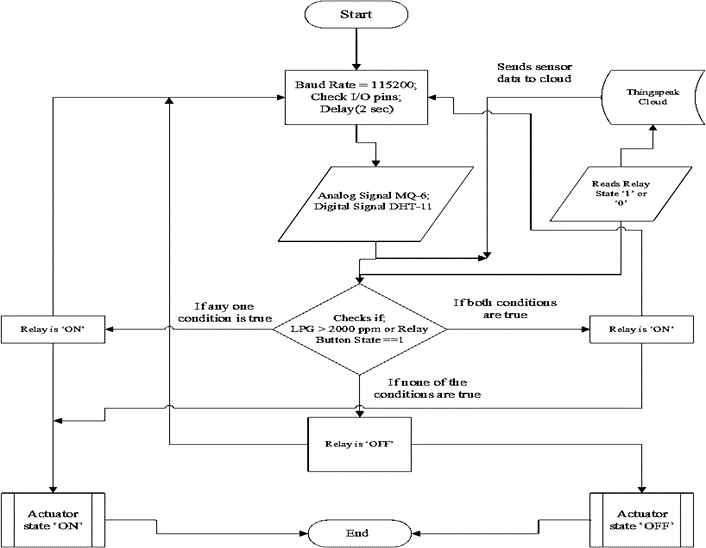
\includegraphics[width=6in,height=6in]{13}
  \caption{Flowchart of the monitoring system}\label{fig13}
\end{figure}
\section{Chapter Summery}
This chapter is about the methods and the algorithm which was used for the system implementation.This chapter contains flowchart with formalized graphic representation of a logic sequence, work process and formalized structure. The purpose of a flow chart is to provide people with a common language or reference point when dealing with a project or process.This Chapter reflects all of this.    